\documentclass[a4paper,english]{ifimaster}

\usepackage[utf8]{inputenc}
\usepackage{babel,duomasterforside}
\usepackage{hyperref}
\usepackage{minted}
\usepackage[backend=biber]{biblatex}

\newcommand{\todo}[1]{\textcolor{red}{[[TODO: #1]]}\PackageWarning{TODO:}{#1!}}
\newcommand{\Fb}{$F_b$}
\newcommand{\FOne}{$F_1$}
\newcommand{\FTwo}{$F_2$}
\newcommand{\Fd}{$F_d$}
\newcommand{\Fm}{$F_m$}
\newcommand{\Es}{$\varepsilon$}
\newcommand{\EsOne}{$\varepsilon_1$}
\newcommand{\EsTwo}{$\varepsilon_2$}

\addbibresource{citations.bib}

\title{Master Essay}
\author{Eirik Halvard Sæther}

\begin{document}

\maketitle
\newpage

\frontmatter{}

\tableofcontents

\mainmatter{}

\chapter{Introduction}%
\label{cha:introduction}

Software engineering methodologies for highly-variable software systems lack support for planning long-term evolution of software. Problems related to the long term evolution planning are more easily detected when you have tools that explicitly model the long term evolution of the software product line. Modelling the evolution of the software product line often involves multiple engineers changing and evolving the plan. Therefor, creating tools for evolution planning requires synchronization techniques for allowing collaborators to merge their partial plans. Naively integrating the changes may yield inconsistencies and conflicts, so we investigate different merging strategies to ensure a sound, well formed plan is produced after the merge.

\section{Motivation}%
\label{sec:motivation}

Feature models are designed to help engineers cope with the long term evolution of software. Designing the software is a iterative and dynamic process, which is subject to change. Having several engineers working in parallel on the same feature model can be beneficial. This requires good tools for handling several engineers working, changing and synchronizing the feature model.

\todo{fix better introduction and motivation, somehow}

\section{Objective}%
\label{sec:objective}

To allow several engineers working in parallel, the goal of this thesis is to design and implement a method of synchronizing and merging the changes from different collaborators on the same feature model. Since the changes from the collaborators were devised from a common feature model, the algorithm should take this common ancestor into consideration when merging, to produce quality results. The algorithm should always produce a syntactically and semantically valid feature model, to ensure a sound, valid feature model as a result. In cases where the merging of the different revisions are not trivial, the method should give ways of resolving conflicts by consulting the user.

\chapter{Background}%
\label{cha:background}

\section{Software product lines}%
\label{sec:software_product_lines}

A software product line (SPL) is a family of closely related software systems. These systems will often have several features in common, as well as variations that makes each piece of software unique. SPLs are used to make highly configurable systems, where each product in the SPL, called a \textit{variant}, is defined by the combination of features chosen.

Software product line engineering is a discipline for efficiently developing such families of software systems. Instead of maintaining potentially hundreds of different software artifacts, these engineering methods have ways of capitalizing on the similarities and differences between each variant. The number of variants are subject to combinatorial explosion, with additions of new features may multiply the amount. Adding new features or fixing bugs can go from updating each variants code base to just updating in one place.

\section{Feature Models}%
\label{sec:feature_models}

All possible variants of a software product line can be defined in terms of a \textit{feature model}. A feature model is a tree structure of features and groups. Features can be manditory or optional, and will contain zero or more groups. Each group has a set of features. A group (of features) can have different types. In example, in an \texttt{AND} group, all the feature has to be chosen.

% Example feature model
\begin{figure}[htpb]
	\centering
	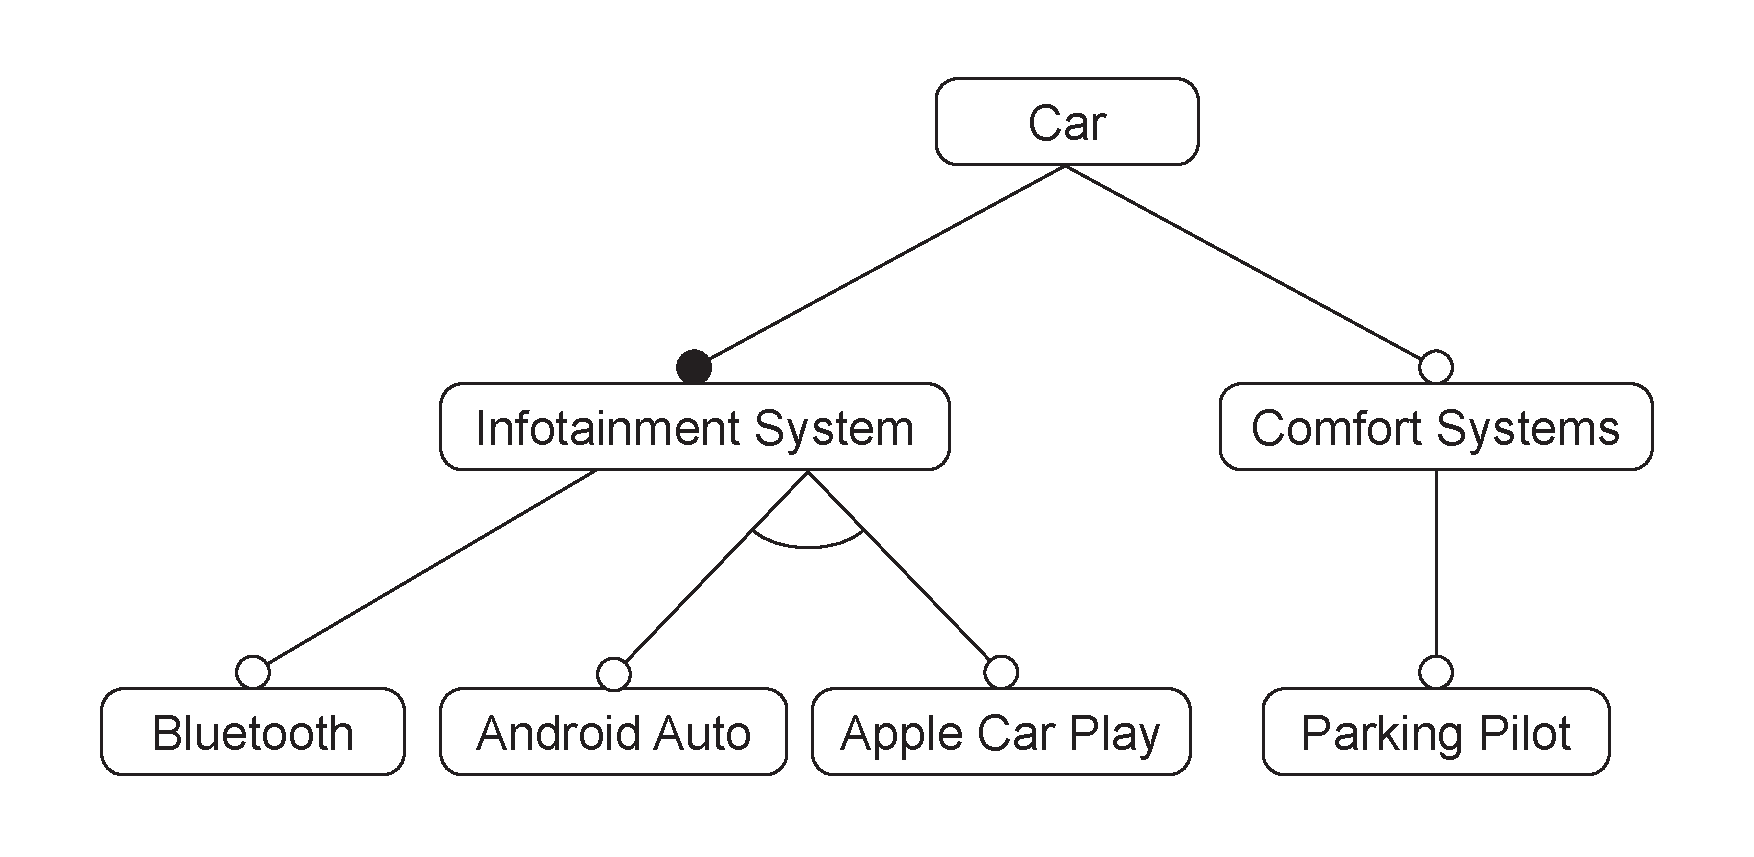
\includegraphics[width=0.8\linewidth]{illustrations/example.pdf}
	\caption{Example feature model}%
	\label{fig:example1}
\end{figure}

A visual representation of a feature model can be seen in Figure~\ref{fig:example1}. The small dot above \texttt{Infotainment System} indicates that the feature is mandatory, where as the white dot above \texttt{Comfort Systems} represents an optional feature. Each feature (except the root) is either implicitly or explicitly in a group. The \texttt{Infotainment System} feature is implicitly in a singleton group below \texttt{Car}. The features \texttt{Android Auto} and \texttt{Apple Car Play} are in a \texttt{XOR} group, indicated by the arch between the features. This represents that each valid variant has to chose between one of the two (but not both).

\section{Evolution planning}%
\label{sec:evolution_planning}

Feature models let engineers capture all variants of the current software product line, but sometimes it can be beneficial to model future or past versions as well. Planning for the long term evolution of the product line can important in managing the complexity that comes with large software systems.

\textit{Evolution plans} lets us model a sequence of feature models, which represents the current and all planned future versions of the feature model. Each feature model represents the product line in a point in time, which could have varying validity, from a week from now to a year. Since the next feature model is derived from the previous one, we can represent the evolution plan as an initial feature model, as well as a sequence of \textit{points}, where each point is a set of operations to perform on the previous feature model to achieve the current one. The operations vary from changing, adding or deleting features or groups from the feature model.

\begin{figure}[htpb]
	\centering
	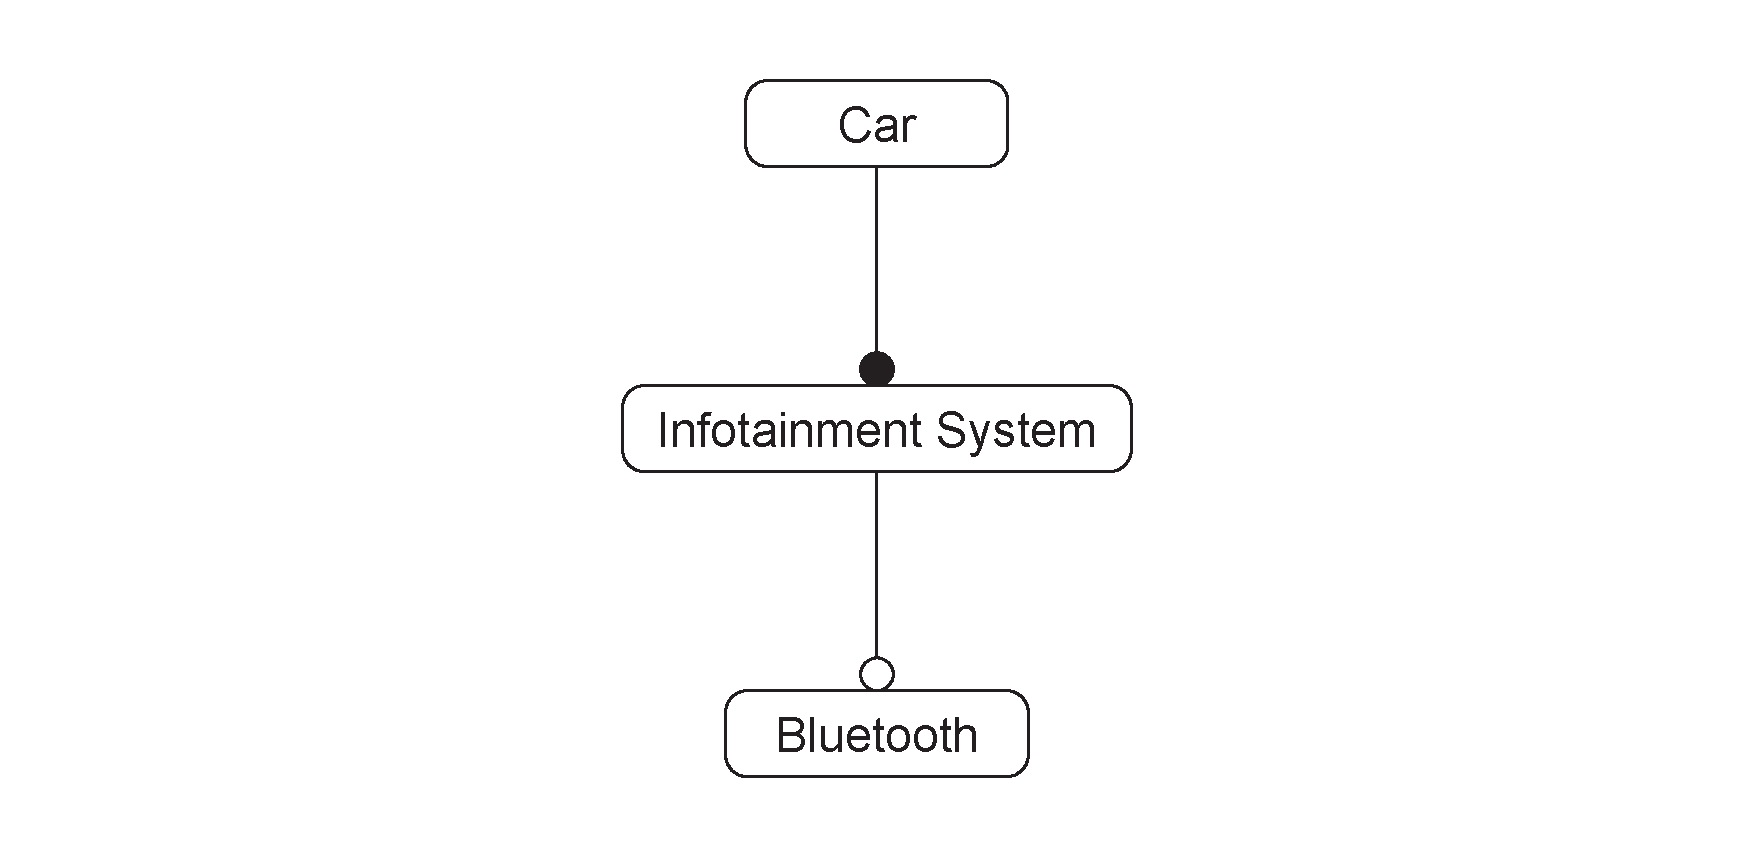
\includegraphics[width=0.8\linewidth]{illustrations/initial.pdf}
	\begin{tabular}{l}
		\textbf{At time 1:}                                           \\ \hline
		add an XOR group to Infotainment System.                      \\
		add feature Android Auto to the Infotainment System XOR group \\
		add feature Car Play to the Infotainment System XOR group     \\
		\\
		\textbf{At time 2:}                                           \\ \hline
		add feature Comfort Systems to the Car AND group              \\
		add an AND group to Comfort Systems                           \\
		add feature Parking Pilot to the Comfort Systems AND group
	\end{tabular}
	\caption{An example evolution plan}%
	\label{fig:exampleplan}
\end{figure}

An example of an evolution plan can be seen in Figure~\ref{fig:exampleplan}. The initial feature model contains three features, and two points have been added. At time 1, a group and two features has been added, an at time 2, another group an two features has been added. The evolution plan can derive three feature models, the initial, and the two at time 1 and 2. When performing all the operations, you will get a feature model that is equal to the one in Figure~\ref{fig:example1}

\section{Version Control Systems}%
\label{sec:version_control_systems}

\textit{Software configuration mechanisms} is the discipline of managing the evolution of large and complex software systems \todo{(61 in~\cite{cite:tom_mens_software_merging_survey})} \textit{Version control mechanisms} \todo{(12 in mens)}, are used to deal with the evolution of software products. These mechanisms include ways to deal with having multiple, parallel versions of the software simultaneously. Techniques like \textit{software merging} are used to keep consistency and unify different versions by automatically or semi-automatically deriving merged versions of the different parallel versions.

Mens~\cite{cite:tom_mens_software_merging_survey} categorizes and describes different aspect of version control systems and software merging techniques. Two-way and three-way merging differentiates between how many versions of the artifact you are comparing. Different representations of the merge artifact can be categorized in textual, syntactic, semantic or structural merging. State-based merge techniques uses delta algorithms to compute differences between revisions while change-based techniques keeps track of the exact operations that were performed between the revisions.

\subsection{Two-way vs three-way merging}%
\label{sub:two_way_vs_three_way_merging}

When merging different versions of a piece of software, we differentiate between \textit{two-way} and \textit{three-way} merging. Two-way merging merges the two versions without taking a common ancestor into account. Three-way merging on the other hand, uses a common ancestor as a reference point, to know how the different versions were changed. The latter technique is more powerful and produces more accurate merges, because the merge will know extra information. Using two-way merge, if a piece was removed from one version, the two-way merge would not know whether the piece was removed in the first file or added in the second. This is not a problem in three-way merge, since we know from the common ancestor whether there was a deletion or addition. In this thesis, we will focus on three-way merging, since it will produce better results.

\subsection{Textual merging}%
\label{sub:textual_merging}

Textual merging views the software artifacts as unstructured text files. There exist several granularities of what is considered one unit, but \textit{line based merging} is probably the most common textual merge. Line based merging techniques computes the difference between files by comparing equality over the lines. This has several implications, like adding a single space after a line is considered a deletion of the old line and addition of the new. This coarse granularity often leads to unnecessary and confusing conflicts. Changing the indentation or other formatting differences often lead to unnecessary conflicts.

To exemplify this, consider the two versions of a python file, Listing~\ref{lst:code_diff_1} and Listing~\ref{lst:code_diff_2}. The second version simply wrapped the content of the function in an if-statement that checks for input sanity. Using a standard textual, line based differencing tool like the Unix' \textit{diff}-tool \todo{ref, see tom for specifics}, we are able calculate the difference between the two files by calculating the longest common subsequence. As seen in the result Listing~\ref{lst:result_code_diff}, difference between the two are confusing and inaccurate. Conceptually, the difference was that the second version wrapped the block in a if-statement. Due to the coarse grained line based differencing and the disregard of structure and semantics, the algorithm reported that the whole block was deleted, and the same block wrapped in an if was inserted.

\begin{listing}
	\begin{minted}[]{python}
def some_function(n):
  sum = 0
  for i in range(0, n):
    sum += i
  print(sum)
some_function(5)

  \end{minted}
	\caption{Code diff 1}
	\label{lst:code_diff_1}
\end{listing}

\begin{listing}
	\begin{minted}[]{python}
def some_function(n):
  if isinstance(n, int):
    sum = 0
    for i in range(0, n):
      sum += i
    print(sum)
some_function(5)
  \end{minted}
	\caption{Code diff 2}
	\label{lst:code_diff_2}
\end{listing}

\begin{listing}
	\begin{minted}{text}
<   sum = 0
<   for i in range(0, n):
<     sum += i
<   print(sum)
---
>   if isinstance(n, int):
>     sum = 0
>     for i in range(0, n):
>       sum += i
>     print(sum)
  \end{minted}
	\caption{Resulting code diff}
	\label{lst:result_code_diff}
\end{listing}

As discussed, text-based merge techniques often provide inferior results, however, they have several advantages. Because of the algorithms focus on generality, accuracy and efficiency, these types of algorithms are widely adopted. The algorithm is general enough to work well for different programming languages, documentation, markup files, configuration files, etc. Some measurements performed on three-way, textual, line-based merge techniques in industrial case studies showed that about 90 percent of the changed files could be merged automatically \todo{ref 49 in mens}. Other tools can complement the merge algorithm in avoiding or resolving conflicts. Formatters can make sure things like indentation and whitespace are uniformly handled, to avoid unnecessary conflicts. Compilers can help in resolving conflicts arising from things like renaming, where one version renames a variables, while another version introduces new lines referencing the old variable.

\subsection{Syntactic Merging}%
\label{sub:syntactic_merging}

Syntactic merging \todo{ref, 10, mens} differs from textual merging in that it considers the syntax of the artifact it is merging. This makes it more powerful, because depending on the syntactic structure of the artifact, the merger can ignore certain aspects, like whitespace or code comments. Syntactic merge techniques can represent the software artifacts in a better data structure than just flat text files, like a tree or a graph. In example, representing the Python program from Listing~\ref{lst:code_diff_1} and Listing~\ref{lst:code_diff_2} as a parse tree or abstract syntax tree, we can avoid merge conflicts. \todo{maybe a nice drawing or something, with explanation}.

The granularity of the merger is still relevant, because we sometimes want to report a conflict even though the versions can be automatically merged. Consider the following example. $n < x$ is changed to $n \leq x$ in one version, and to $n < x + 1$ in another. Too fine grained granularity may cause this to be merged conflict free as $n \leq x + 1$. The merge can be done automatically and conflict free, but here we want to report a warning or conflict, because the merge might lead to logical errors.

\subsection{Semantic Merging}%
\label{sub:semantic_merging}

While syntactic merging is more powerful than its textual counterpart, there are still conflicts that go unnoticed. The syntactical mergers can detect conflicts explicitly encoded in the tree structure of the software artifact, however, there often exist implicit, cross-tree constraints in the software. An example of such a constraint is references to a variable. The variable references in the code are often semantically tied to the definition of the variable, where the name and scope implicitly notes the cross tree reference to the definition.

Consider the following simple program: \texttt{var i; i = 10;}. If one version changes the name of the variable: \texttt{var num; num = 10;}, and another version adds a statement referencing the variable: \texttt{var i; i = 10; print(i)}. Syntactic or textual mergers would not notice the conflict arising due to the implicit cross-tree constraints regarding the variable references, and merge the versions conflict-free with the following, syntactically valid result: \texttt{var num; num = 10; print(i)}.

Semantic mergers takes these kinds of conflicts into consideration while merging. Using \textit{Graph-based}  or \textit{context-sensitive} merge techniques, we can model such cross tree constraints, by linking definitions and invocations with edges in the graph. However, in some cases, such \textit{static semantic} merge techniques are not sufficient. Some changes cannot generally be detected statically, and may need to rely on the runtime semantics.

\chapter{A sound merging strategy for evolution plans}%
\label{cha:solution}

\section{Goal of the thesis}%
\label{sec:goal_of_the_thesis}

As described in Section~\ref{sec:evolution_planning}, having tools that help model the long term evolution of SPLs can help manage the complexity and difficulty in development. Especially in larger systems, several persons and teams often work independently on the same software product line, but on different assets. Tools that help evolution planning would benefit from having ways of merging and synchronizing different versions of the evolution plan.

This thesis will focus on developing a three-way merging technique (see Section~\ref{sub:two_way_vs_three_way_merging}) for merging two evolution plans in respect to a common previous evolution plan which the two versions were derived from. In some cases, the changes made to the evolution plan are disjoint, which will result in a conflict free merge. In other cases, naively merging the two plans might result in an unsound and invalid evolution plan. The merge algorithm should detect these cases, and report what cases caused inconsistencies. While detecting conflicts is good, it would be even better if the algorithm provided ways of fixing the conflicts. This can be done in many ways, but a good technique for conflict fixing should have a good balance between usability, complexity and accuracy. But most importantly, the algorithm should result in a sound, well formed evolution plan.

\section{Why existing solutions are not adequate}%
\label{sec:why_existing_solutions_are_not_adequate}

While there are several tools to handle three-way merging, they do not produce adequate results to solve the problem. Tools such as diff \todo{github, unix, ref} are one of the most used tools for the task, due to their generality and efficiency. However, due to the algorithm being just a line based, textual merger (see Section~\ref{sub:textual_merging}), much of the structure will get lost in the result, leading to an invalid evolution plan.

One could also consider a syntactic/structural merger (Section~\ref{sub:syntactic_merging}, which would take the structure of the software artifact into consideration. There exist several syntactic mergers already, like the three-way XML merger proposed by Lindholm~\cite{cite:lindholm_xml_merge}. One could try to encode the evolution plans in an XML structure, and merge the results. This would eliminate a lot of the structural merge problems that occur using textual mergers like unix diff. 

However, several of the more implicit semantic requirements of evolution plans could go unnoticed in the merge result, producing a invalid evolution plan without the algorithm giving any warnings. This could happen if each version moves a node to a descendant of the other node, creating a cycle. Feature models also have requirements like features in groups with type \texttt{XOR} or \texttt{OR} cannot be mandatory, which can easily be violated when merging the changed plans. There are also several other potential issues when merging the evolution plans.

While detecting the conflicts is one issue, dealing with them is another. Merging the results can lead to conflicting operations which would need to be dealt with. The algorithm should deal with this in a usable, clear manner. Customizing and tailoring the algorithm would potentially help deal with this.

Merging evolution plans is no trivial task, because the structure and semantics will have to be carefully considered in the merge. To ensure the merge results in a sound evolution plan, we cannot rely on existing algorithms.

\section{Difficulties and potential solutions}%
\label{sec:difficulties_and_potential_solutions}

suitable Representation for FM and EP

things to consider. granularity, easy to understand for user.

cascading warnings?
incrementally produce merged plan. this lets engineer make sure semantics and core of the plan is still good.
globally merge would make this more difficult in complexity and usability. Possibly also too hard. 
Potentially identify when things have to be in place, (dependencies between operations, etc)
fikse og ordne warnings mens man går fremover. noen paradokser kan potensielt utsettes til slutt?
dead operations. sletting av noder som er borte.
potensielle problemer med inkrementell. node slettes i 1 og 2, den første vil bli prioritert.
analysere gjennom først? trickery er det uansett.
ting som er vanskelig og byr på problemer skriver vi om i difficulties

When you move a feature to another part of the tree, and then modify the name, general algorithms would not know if you deleted a feature and created a new, or if you moved and changed the same feature. However, due to the well defined semantics of feature models, we know that every feature has a unique identifier, which can be leveraged by the merge algorithm.


\section{Difficulties and challenges}%
\label{sec:difficulties_challenges}

Evolution plan merging is not trivial, and different merging techniques and evolution plan representations will have advantages and disadvantages in terms of usability, complexity and accuracy.

\subsection{Feature model representations}%
\label{sub:feature_model_representations}

Since a feature model is a tree structure consisting of features and groups, it would be natural to represent this as a standard (mutually) recursive tree structure of features and groups. However, since we know that each feature and group are uniquely identified by an id, we can define the feature model as a map from identifier to feature. This is beneficial for merging, for example when we are moving a feature. Instead of traversing the tree several times, where we can simply update the parent of one of the mappings.

\subsection{Evolution plan representations}%
\label{sub:evolution_plan_representations}

An evolution plan is simply just a list of feature models, with each feature model associated with a time point. Each feature model acts as a snapshot of what the intended product line should look like at the specified time point. In this representation, the operations performed between each step is implicit.

Evolution plans could also be represented by explicitly deriving the operations between the each adjacent feature model. This can be modelled as an initial feature model, and a list of \textit{points}, where each point consists of a time point and a list of operations. The points represents what changes are intended to take place during a certain time point. The feature model for each time point can then be calculated by applying the operations to the feature model.

Another approach is modelling everything with validities. Instead having add and remove features operations at different time points, each feature can be encoded with a start and (optional) end time. Each feature and group can have an interval of existence, which can be utilized by a merge algorithm.

\subsection{Merging strategies}%
\label{sub:merging_strategies}

How the evolution plan is represented will affect how the merge is performed.

\todo{say something about incremental merging. problems there}

\todo{say something about simultaneous. plan can be seen as a whole. May result in more accurate results/conflicts where a feature is removed at different time points in the two plans. problems there might include ensuring a well formed evolution plan}


\section{Notation}%
\label{sec:notation}

Throughout this thesis, I will use the following variable naming convention. Let \Fb{} be the initial base feature model, while \FOne{} and \FTwo{} be two different feature models, derived from model \Fb{}. To note either of the two derived ones, we use the notation $F_d$. We call the resulting feature model after the merge algorithm is performed \Fm{}.

The edit script, which is the calculated list of operations to go from \Fb{} to one of the derived models \Fd{}, we note as \Es{}. If we need to be specific to which of the derived models were computed, we note this with \EsOne{} and \EsTwo{}.

\section{Feature model semantics}%
\label{sec:feature_model_semantics}

Definitions of feature models, groups, etc. Taken from the paper stuff \todo{write}

\section{Change detection}%
\label{sec:change_detection}

One step of computing \Fm{} from \Fb{}, \FOne{} and \FTwo{}, is computing the two edit scripts \EsOne{} and \EsTwo{}. The edit scripts are computed by a directed delta algorithm \cite{cite:tom_mens_software_merging_survey}. The delta algorithm has three distinct phases. (1) The algorithm will compute the difference between \Fb{} and \Fd{}, and produce a set of operations (See the operation table \ref{tab:list_of_operations}) needed to get from the base to the derived model. (2) The necessary operations and dependencies between the operations are modeled in a dependency graph. This is due to certain operations needing to be performed before others, i.e. every child has to be removed before you can remove the parent. (3) A topological sorting is performed on the graph to compute an ordered list of operations. When performing the operations in order starting with \Fb{}, the resulting feature model will be equal to the actual derived one. This eliminates the need to track and log the operations when they are being performed by a user. \todo{not actually what is going to happen I think}


\begin{table}[htpb]
	\centering
	\caption{List of operations}
	\label{tab:list_of_operations}
	\begin{tabular}{c}
		\todo{make as table}
	\end{tabular}
	\begin{itemize}
		\item Add feature
		\item Add group
		\item Move feature to group
		\item Move group to feature
		\item Delete feature
		\item Delete group
		\item Change feature
		\item Change group
	\end{itemize}
\end{table}

\subsection{Dependencies between merge changes}%
\label{sub:dependencies_between_merge_changes}

\subsubsection{Cycle Detection}%
\label{ssub:cycle_detection}

Based on the assumption that the base \Fb{}, and the derived feature models, \FOne{} and \FTwo{} are valid and sound feature models, we know that they contain no cycles. However, when synthesising the merged model, cycles can occur if both edit scripts contain move operations. If \EsOne{} contains \texttt{MoveFeature(Fid, Gid)}, and \EsTwo{} contains \texttt{MoveFeature(Fid', Gid')}, we need to ensure that integrating the changes doesn't produce any cycles. If \texttt{Fid} is moved to \texttt{Gid}, problems can occur if \texttt{Fid'} now becomes the new ancestor of \texttt{Fid} and \texttt{Gid'} is a subgroup of \texttt{Fid}.

\chapter{Roadmap}%
\label{cha:roadmap}

\chapter{Unused (will be removed)}%
\label{cha:unused_will_be_removed_}

\section{Related Work}%
\label{sec:related_work}

\subsection{A Three-way Merge for XML Documents}%
\label{sub:_a_three_way_merge_for_xml_documents}

Lindholm describes a method of merging XML documents. The algorithm is a three-way merge taking a base XML file, $T_0$, and two files $T_1$ and $T_2$, derived and changed from the base file independently. The XML documents are ordered, labeled trees, and merging the trees takes this into consideration. The algorithm relies on computing \textit{edit scripts} between $T_0$ and $T'$, where $T'$ is either $T_1$ or $T_2$. The edit scripts consist of predefined operations, which are attribute updates and insert, move and delete for XML elements.

One of the important factors of the data structure, is that the nodes are labeled with unique IDs. This makes merging significantly easier.

To study different use-cases (user stories) of XML merging, they manually merged some examples, to see how real world users would handle some tricky cases. Some rules for merging were devised, including:

\begin{itemize}
	\item Not possible to move a node in $T_1$ that are being updated in $T_2$
	\item Guards, aka node contexts are there to handle merging changes originating too close to each other. This isn't technically a merge conflict, but a potential semantic issue.
	\item Normal stuff. Added or removed nodes should be reflected in the merge. Parent relation should be updated
\end{itemize}

% TODO: check reference 2 and 3 in the text, regarding matching/mapping and the tree matching problem

possible a paragraph about different version control mechanisms and techniques. Pessimistic and optimistic approaches. \cite{cite:tom_mens_software_merging_survey}

Introduce a method of merging two feature models derived from the same feature model using a three-way merge algorithm inspired from the text-granularity algorithm and other three-way merge algorithms working on tree-structures like XML and ASTs.

These solutions are not adequate, because we want to create an algorithm that ensures soundness and takes the semantics of feature models into account when merging. This task is not trivial, and the use cases of the developers will need to be considered when deciding which conflicts to automatically merge, warn the user, etc. The algorithm will utilize properties about feature models when merging, like the fact that the nodes are unordered, and each node is uniquely identified by their id.

This task includes defining the semantics of feature models, defining what a sound model is. The three-way merge algorithm will assume three sound feature models as input, and compute the edit script between the base and the two derived feature models. The two edit scripts will then be combined to a graph that represents what changes to be done to the base, including possible conflicts and dependencies.

\section{A State-of-the-Art Survey on Software Merging}%
\label{sec:a_state_of_the_art_survey_on_software_merging}

% TODO: read Tom Mens survey on software merging


\backmatter{}

\printbibliography{}

\end{document}
